\documentclass{standalone}
\usepackage{tikz}
\usetikzlibrary{patterns, positioning}


\begin{document}
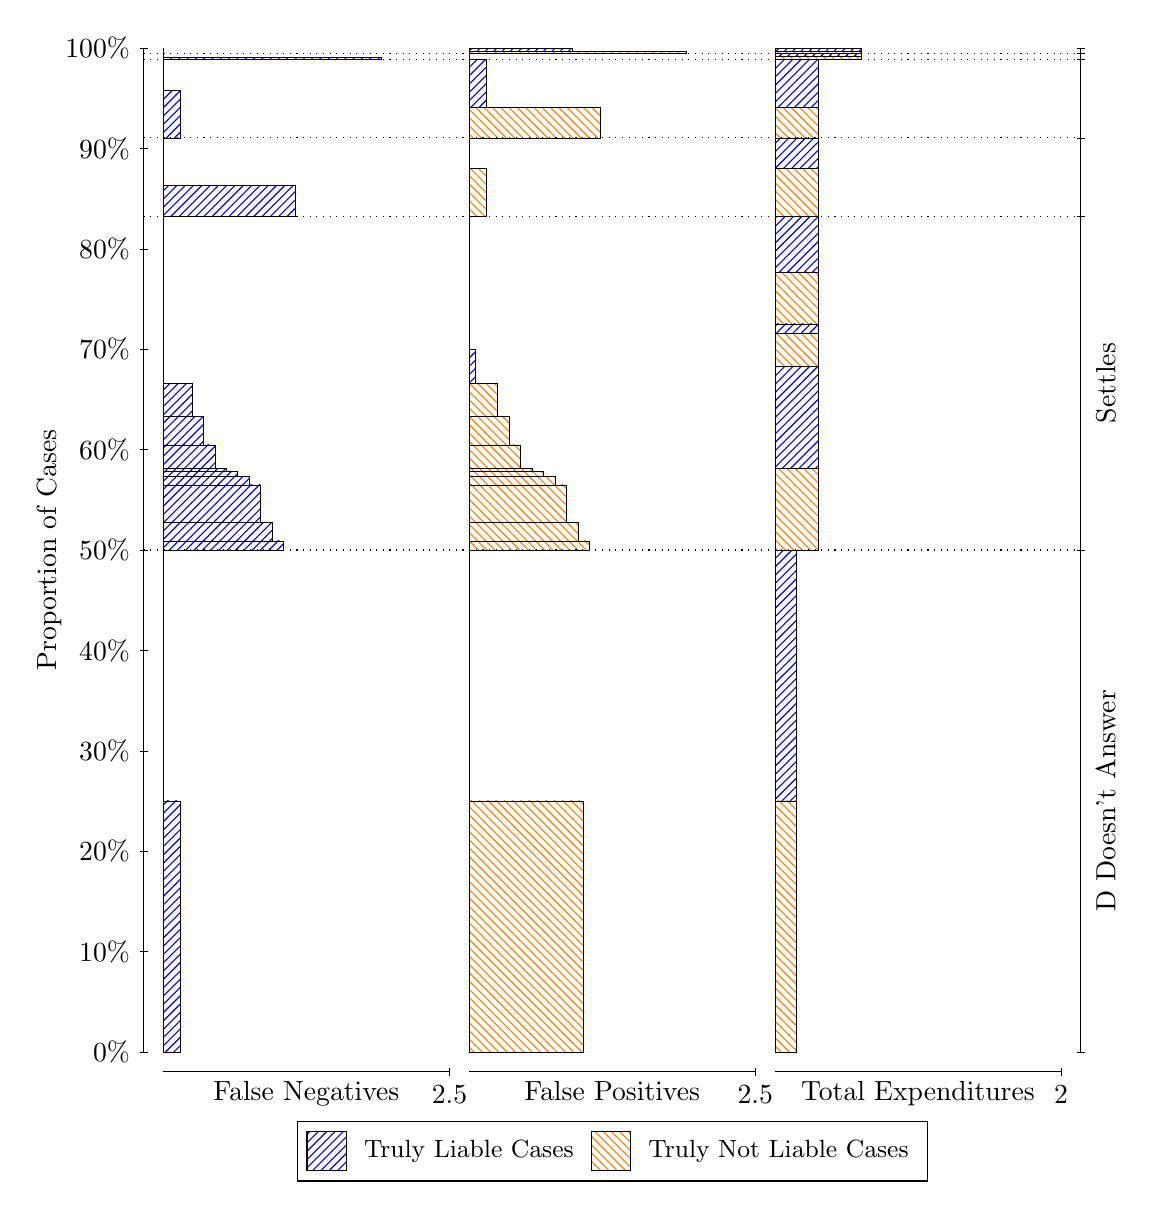
\begin{tikzpicture}
\draw[black, very thin] (1.5,1.75) -- (1.5,14.5);
\node[rotate=90, text=black, anchor=center] at (0.3, 8.125) {Proportion of Cases};
\draw[black, very thin] (1.45,1.75) -- (1.55,1.75);
\node[text=black, anchor=east] at (1.45, 1.75) {0\%};
\draw[black, very thin] (1.45,3.025) -- (1.55,3.025);
\node[text=black, anchor=east] at (1.45, 3.025) {10\%};
\draw[black, very thin] (1.45,4.3) -- (1.55,4.3);
\node[text=black, anchor=east] at (1.45, 4.3) {20\%};
\draw[black, very thin] (1.45,5.575) -- (1.55,5.575);
\node[text=black, anchor=east] at (1.45, 5.575) {30\%};
\draw[black, very thin] (1.45,6.85) -- (1.55,6.85);
\node[text=black, anchor=east] at (1.45, 6.85) {40\%};
\draw[black, very thin] (1.45,8.125) -- (1.55,8.125);
\node[text=black, anchor=east] at (1.45, 8.125) {50\%};
\draw[black, very thin] (1.45,9.4) -- (1.55,9.4);
\node[text=black, anchor=east] at (1.45, 9.4) {60\%};
\draw[black, very thin] (1.45,10.675) -- (1.55,10.675);
\node[text=black, anchor=east] at (1.45, 10.675) {70\%};
\draw[black, very thin] (1.45,11.95) -- (1.55,11.95);
\node[text=black, anchor=east] at (1.45, 11.95) {80\%};
\draw[black, very thin] (1.45,13.225) -- (1.55,13.225);
\node[text=black, anchor=east] at (1.45, 13.225) {90\%};
\draw[black, very thin] (1.45,14.5) -- (1.55,14.5);
\node[text=black, anchor=east] at (1.45, 14.5) {100\%};

\draw[black, very thin] (13.4,1.75) -- (13.4,14.5);
\draw[black, very thin] (13.35,1.75) -- (13.45,1.75);
\node[anchor=west] at (13.35, 1.75) {};
\draw[black, very thin] (13.35,8.125) -- (13.45,8.125);
\node[anchor=west] at (13.35, 8.125) {};
\draw[black, very thin] (13.35,12.365) -- (13.45,12.365);
\node[anchor=west] at (13.35, 12.365) {};
\draw[black, very thin] (13.35,13.36) -- (13.45,13.36);
\node[anchor=west] at (13.35, 13.36) {};
\draw[black, very thin] (13.35,14.355) -- (13.45,14.355);
\node[anchor=west] at (13.35, 14.355) {};
\draw[black, very thin] (13.35,14.428) -- (13.45,14.428);
\node[anchor=west] at (13.35, 14.428) {};
\draw[black, very thin] (13.35,14.5) -- (13.45,14.5);
\node[anchor=west] at (13.35, 14.5) {};

\draw[black, very thin, pattern color=blue, pattern=north east lines] (1.75,1.75) rectangle (1.968,4.9375);
\draw[black, very thin, pattern color=orange, pattern=north west lines] (1.75,4.9375) rectangle (1.75,8.125);
\draw[black, very thin, pattern color=blue, pattern=north east lines] (1.75,8.125) rectangle (3.276,8.242);
\draw[black, very thin, pattern color=blue, pattern=north east lines] (1.75,8.242) rectangle (3.1307,8.4787);
\draw[black, very thin, pattern color=blue, pattern=north east lines] (1.75,8.4787) rectangle (2.9853,8.9513);
\draw[black, very thin, pattern color=blue, pattern=north east lines] (1.75,8.9513) rectangle (2.84,9.0611);
\draw[black, very thin, pattern color=blue, pattern=north east lines] (1.75,9.0611) rectangle (2.6947,9.1227);
\draw[black, very thin, pattern color=blue, pattern=north east lines] (1.75,9.1227) rectangle (2.5493,9.1591);
\draw[black, very thin, pattern color=blue, pattern=north east lines] (1.75,9.1591) rectangle (2.404,9.4613);
\draw[black, very thin, pattern color=blue, pattern=north east lines] (1.75,9.4613) rectangle (2.2587,9.8182);
\draw[black, very thin, pattern color=blue, pattern=north east lines] (1.75,9.8182) rectangle (2.1133,10.245);
\draw[black, very thin, pattern color=orange, pattern=north west lines] (1.75,10.245) rectangle (1.75,12.365);
\draw[black, very thin, pattern color=blue, pattern=north east lines] (1.75,12.365) rectangle (3.4213,12.756);
\draw[black, very thin, pattern color=orange, pattern=north west lines] (1.75,12.756) rectangle (1.75,13.36);
\draw[black, very thin, pattern color=blue, pattern=north east lines] (1.75,13.36) rectangle (1.968,13.964);
\draw[black, very thin, pattern color=orange, pattern=north west lines] (1.75,13.964) rectangle (1.75,14.355);
\draw[black, very thin, pattern color=blue, pattern=north east lines] (1.75,14.355) rectangle (4.5113,14.382);
\draw[black, very thin, pattern color=orange, pattern=north west lines] (1.75,14.382) rectangle (1.75,14.428);
\draw[black, very thin, pattern color=orange, pattern=north west lines] (1.75,14.428) rectangle (1.75,14.455);
\draw[black, very thin, pattern color=blue, pattern=north east lines] (1.75,14.455) rectangle (1.75,14.5);
\draw[black, very thin, pattern color=orange, pattern=north west lines] (5.6333,1.75) rectangle (7.0867,4.9375);
\draw[black, very thin, pattern color=blue, pattern=north east lines] (5.6333,4.9375) rectangle (5.6333,8.125);
\draw[black, very thin, pattern color=orange, pattern=north west lines] (5.6333,8.125) rectangle (7.1593,8.242);
\draw[black, very thin, pattern color=orange, pattern=north west lines] (5.6333,8.242) rectangle (7.014,8.4787);
\draw[black, very thin, pattern color=orange, pattern=north west lines] (5.6333,8.4787) rectangle (6.8687,8.9513);
\draw[black, very thin, pattern color=orange, pattern=north west lines] (5.6333,8.9513) rectangle (6.7233,9.0611);
\draw[black, very thin, pattern color=orange, pattern=north west lines] (5.6333,9.0611) rectangle (6.578,9.1226);
\draw[black, very thin, pattern color=orange, pattern=north west lines] (5.6333,9.1226) rectangle (6.4327,9.1591);
\draw[black, very thin, pattern color=orange, pattern=north west lines] (5.6333,9.1591) rectangle (6.2873,9.4612);
\draw[black, very thin, pattern color=orange, pattern=north west lines] (5.6333,9.4612) rectangle (6.142,9.8181);
\draw[black, very thin, pattern color=orange, pattern=north west lines] (5.6333,9.8181) rectangle (5.9967,10.245);
\draw[black, very thin, pattern color=blue, pattern=north east lines] (5.6333,10.245) rectangle (5.706,10.672);
\draw[black, very thin, pattern color=blue, pattern=north east lines] (5.6333,10.672) rectangle (5.6333,12.365);
\draw[black, very thin, pattern color=orange, pattern=north west lines] (5.6333,12.365) rectangle (5.8513,12.969);
\draw[black, very thin, pattern color=blue, pattern=north east lines] (5.6333,12.969) rectangle (5.6333,13.36);
\draw[black, very thin, pattern color=orange, pattern=north west lines] (5.6333,13.36) rectangle (7.3047,13.751);
\draw[black, very thin, pattern color=blue, pattern=north east lines] (5.6333,13.751) rectangle (5.8513,14.355);
\draw[black, very thin, pattern color=orange, pattern=north west lines] (5.6333,14.355) rectangle (5.6333,14.401);
\draw[black, very thin, pattern color=blue, pattern=north east lines] (5.6333,14.401) rectangle (5.6333,14.428);
\draw[black, very thin, pattern color=orange, pattern=north west lines] (5.6333,14.428) rectangle (8.3947,14.455);
\draw[black, very thin, pattern color=blue, pattern=north east lines] (5.6333,14.455) rectangle (6.9413,14.5);
\draw[black, very thin, pattern color=orange, pattern=north west lines] (9.5167,1.75) rectangle (9.7892,4.9375);
\draw[black, very thin, pattern color=blue, pattern=north east lines] (9.5167,4.9375) rectangle (9.7892,8.125);
\draw[black, very thin, pattern color=orange, pattern=north west lines] (9.5167,8.125) rectangle (10.062,9.1591);
\draw[black, very thin, pattern color=blue, pattern=north east lines] (9.5167,9.1591) rectangle (10.062,10.453);
\draw[black, very thin, pattern color=orange, pattern=north west lines] (9.5167,10.453) rectangle (10.062,10.879);
\draw[black, very thin, pattern color=blue, pattern=north east lines] (9.5167,10.879) rectangle (10.062,10.996);
\draw[black, very thin, pattern color=orange, pattern=north west lines] (9.5167,10.996) rectangle (10.062,11.656);
\draw[black, very thin, pattern color=blue, pattern=north east lines] (9.5167,11.656) rectangle (10.062,12.365);
\draw[black, very thin, pattern color=orange, pattern=north west lines] (9.5167,12.365) rectangle (10.062,12.969);
\draw[black, very thin, pattern color=blue, pattern=north east lines] (9.5167,12.969) rectangle (10.062,13.36);
\draw[black, very thin, pattern color=orange, pattern=north west lines] (9.5167,13.36) rectangle (10.062,13.751);
\draw[black, very thin, pattern color=blue, pattern=north east lines] (9.5167,13.751) rectangle (10.062,14.355);
\draw[black, very thin, pattern color=orange, pattern=north west lines] (9.5167,14.355) rectangle (10.607,14.401);
\draw[black, very thin, pattern color=blue, pattern=north east lines] (9.5167,14.401) rectangle (10.607,14.428);
\draw[black, very thin, pattern color=orange, pattern=north west lines] (9.5167,14.428) rectangle (10.607,14.455);
\draw[black, very thin, pattern color=blue, pattern=north east lines] (9.5167,14.455) rectangle (10.607,14.5);
\draw[black, dotted] (1.5,8.125) -- (13.4,8.125);
\draw[black, dotted] (1.5,12.365) -- (13.4,12.365);
\draw[black, dotted] (1.5,13.36) -- (13.4,13.36);
\draw[black, dotted] (1.5,14.355) -- (13.4,14.355);
\draw[black, dotted] (1.5,14.428) -- (13.4,14.428);
\draw[black, very thin] (1.75,1.5) -- (5.3833,1.5);
\node[text=black, anchor=north] at (3.5667, 1.5) {False Negatives};
\draw[black, very thin] (5.3833,1.45) -- (5.3833,1.55);
\node[text=black, anchor=north] at (5.3833, 1.45) {2.5};

\draw[black, very thin] (5.6333,1.5) -- (9.2667,1.5);
\node[text=black, anchor=north] at (7.45, 1.5) {False Positives};
\draw[black, very thin] (9.2667,1.45) -- (9.2667,1.55);
\node[text=black, anchor=north] at (9.2667, 1.45) {2.5};

\draw[black, very thin] (9.5167,1.5) -- (13.15,1.5);
\node[text=black, anchor=north] at (11.333, 1.5) {Total Expenditures};
\draw[black, very thin] (13.15,1.45) -- (13.15,1.55);
\node[text=black, anchor=north] at (13.15, 1.45) {2};

\node[text=black, centered, rotate=90] at (13.72, 4.9375) {D Doesn't Answer};
\node[text=black, centered, rotate=90] at (13.72, 10.245) {Settles};





\draw (7.449999999999999,1.5) node[draw=none] (baseCoordinate) {};
\begin{scope}[align=center]
        \matrix[scale=0.5, draw=black, below=0.5cm of baseCoordinate, nodes={draw}, column sep=0.1cm]{
            \node[rectangle, draw, minimum width=0.5cm, minimum height=0.5cm, pattern color=blue, pattern=north east lines] {}; &
            \node[draw=none, font=\small, text=black] (B) {Truly Liable Cases}; &
            \node[rectangle, draw, minimum width=0.5cm, minimum height=0.5cm, pattern color=orange, pattern=north west lines] {}; &
            \node[draw=none, font=\small, text=black] (B) {Truly Not Liable Cases}; \\
            };
\end{scope}

\end{tikzpicture}
\end{document}